%----------------------------------------------------------------
% FEUILLE DE STYLE ENSG au format Latex
% Création : sept. 2010 (D Lercier)
% Modification sept. 2012 (T Coupin)
%----------------------------------------------------------------

\documentclass{themeensg}

%---Texte en filigranne---
%pour l'enlever : \SetWatermarkText{}
%-------------------------

%---Mes packages à moi---
%\usepackage{}
%------------------------

%---Mes raccourcis---
\newcommand{\transpose}[1]{{}^t \! #1}
\newcommand{\ensg}{\textsc{Ensg}}
%--------------------

%---Paramètres du pdf---
    \hypersetup{
       backref=true,                           % Permet d'ajouter des liens dans
       pagebackref=true,                       % les bibliographies
       hyperindex=true,                        % Ajoute des liens dans les index.
       colorlinks=true,  %Colorise les liens : true pour version numérique, false pour version d'impression
       breaklinks=true,                        % Permet le retour à la ligne dans les liens trop longs.
       urlcolor= blue,                         % Couleur des hyperliens.
       linkcolor= blue,                       % Couleur des liens internes.
       bookmarks=true,                         % Créé des signets pour Acrobat.
       %bookmarksopen=true,                    % Si les signets Acrobat sont créés,
                                               % les afficher complètement.
       pdftitle={Thème ENSG},                 % Titre du document.
                                               % Informations apparaissant dans
       pdfauthor={Thibault Coupin},                      % dans les informations du document
       pdfsubject={Feuille de style ENSG}           % sous Acrobat.
    }

%-----------------------



%-------------------------------------------------------------

\setcounter{tocdepth}{1} %profondeur de la table des matières

\title{Feuille de style \LaTeX~de l'\ensg\\Documentation plus que rapide\\Version provisoire du \today~à \timenow}

%
%-------------------------------------------------------------
% Début du document
%--------------------------------------------------------------
\begin{document}
%--------------------------------------------------------------
\begin{titlepage}
%Inclusion des labels des entreprises
%Pour un seul label (à gauche), mettre NULL pour les 3e et 4e argument
\enterprise 
{logos/logo_ensg.jpg}
{Ecole Nationale des Sciences Géographiques}
{logos/logo_ensg.jpg}
{Ecole Nationale des Sciences Géographiques}

%Inclusion du titre
\maketitle{Stage de fin d'études \\Cycle des Ingénieurs diplômés de l'ENSG 3\up{ème} année }{logos/logo_ensg.jpg}

\infos{Mohamed-Amjad LASRI}{Septembre 2015}
\end{titlepage}


%---Page du jury---
%---Page du jury---
\newevenpage
\thispagestyle{plain}
\section*{Jury}
\vspace{0.5cm}

\textbf{Président de jury :} \\

Pierre-Yves Hardouin, directeur des enseignements de l'ENSG

\vspace{0.5cm}

\textbf{Commanditaire :} \\

KYLIA


Laboratoire d’Opto-Electronique, Métrologie et Instrumentation (LOEMI), Institut de l’Information Géographique et Forestière (IGN)

\vspace{0.5cm}

\textbf{Encadrement de stage :} \\ 

Olivier Martin IGN/DRE/SRSIG/LOEMI

Frédéric Verluise KYLIA

Emmanuel Bardière ENSG

\vspace{0.5cm}

\textbf{Responsable pédagogique du cycle Ingénieur :} \\

Serge Botton, IGN/ENSG/DE/DPTS

\vspace{0.5cm}

\textbf{Tuteur du stage pluridisciplinaire :} \\

Patricia Parisi, IGN/ENSG/DE/DSHI

\vspace{1cm}

\copyright \hspace{0.3cm} ENSG

\section*{Stage de fin d'étude du 04/05/2015 au 04/10/2015 }
\vspace{0.3cm}
\textbf{Diffusion web :} $\boxtimes$ Internet \hspace{0.2cm}$\boxtimes$ Intranet Polytechnicum\hspace{0.2cm}
$\boxtimes$ Intranet ENSG\vspace{0.3cm}

\textbf{Situation du document :} 
\vspace{0.2cm}
\par
Rapport de stage de fin d'études présenté en fin de 3\up{ème} année du cycle des Ingénieurs
\vspace{0.3cm}


\newcounter{x}
\setcounter{x}{\getpagerefnumber{LastPage}-\getpagerefnumber{beginappendices}+1}

\textbf{Nombres de pages :} 50 pages dont 3 d'annexes
\vspace{0.3cm}

\textbf{Système hôte :} \LaTeX
\vspace{1cm}


\textbf{Modifications :} 
\begin{center}
\begin{tabular}{|c|c|c|>{\centering}p{6.5cm}|}
\hline 
EDITION & REVISION & DATE & PAGES MODIFIEES\tabularnewline
\hline
\hline 
1 & 0 & 09/2015 & Création\tabularnewline
\hline 

\end{tabular}
\end{center}
%------------------

%------------------------------------------------------------------------------
% Remerciements
%\newevenpage
\chapter*{Remerciements}

Je tiens à remercier toutes les personnes qui ont participé de différentes façons à la réussite de mon stage et plus particulièrement les personnes que je cite ci-dessous.

Olivier MARTIN, Frederic VERLUISE, Christian THOM et Christophe MEYNARD qui m'ont encadré, conseillé et ont répondu régulièrement à mes questions tout au long de mon stage.

Emmanuel BARDIERE, mon référent de stage ENSG, qui a suivi l'évolution de mon stage tout au long de ces cinq mois.

Tout le personnel du Laboratoire d'Opto-Électronique et de la société KYLIA.



%---Résumé (français)---
\begin{abstract}
\thispagestyle{empty}
	\vspace{1cm}

	Ceci est mon résumé
	
	\vspace{1.5cm}
	
	\textbf{Mots clés :} clés, clés, clés
\end{abstract}
%-----------------------


%---Résumé (anglais)---
\selectlanguage{english}
\begin{abstract}
\thispagestyle{empty}
	\vspace{1cm}
	
	This is my abstract
	
	\vspace{1.5cm}
	
	\textbf{Key words:} key, key, key
\end{abstract}
%----------------------

\selectlanguage{frenchb}

%---Table des matières, des figures et des tableaux---
%\newevenpage
\tableofcontents

\newevenpage
\listoffigures

\newevenpage
\listoftables
%----------------------------------------------------

%\newevenpage
\chapter*{Glossaire et sigles utiles}
\addcontentsline{toc}{chapter}{Glossaire et sigles utiles}

  \begin{acronym}
  \acro{ENSG}{\'Ecole Nationale des Sciences Géographiques}
  \acro{FIFO}{First In First Out}
  \acro{G3OS}{Geocube Operating System}
  \acro{GNSS}{Global Navigation Satellite Systems}
  \acro{GPS}{Global Positionning System}
  \acro{IEC}{The International Electrotechnical Commission}
  \acro{IHM}{Interface Homme Machine}
  \acro{ISO}{The International Organization for Standardization}
  \acro{NFC}{Near Field Communication}
  \acro{PCD}{Proximity Coupling Device}
  \acro{PICC}{Proximity Inductive Coupling Card}
  \acro{RTOS}{Real Time Operating System}
  \acro{TCP/IP}{Transmission Control Protocol/Internet Protocol}
  \end{acronym}


%---Introduction------------------------------------------------------------------
\newevenpage
\chapter*{Introduction}
  \addcontentsline{toc}{chapter}{Introduction}
  
  \vspace{1.5cm}
  
	La communication en champ proche (NFC) est une méthode de communication utilisée pour l'identification des personnes et des objets

%-------------------------------------------------------------------------------

\evenchapter[Concepts clés et problématiques]{Concepts clés et problématiques}

\textit{ Ce chapitre a pour but d'introduire le lecteur aux concepts clés nécessaires pour comprendre le travail effectué lors de ce stage.
Le lecteur est prié de prêter une attention particulière au tableau des sigles lors de la lecture du présent document. Les protocoles qu'on présente utilisent un certain nombre d’abréviations conventionnelles pour désigner Les opérations d'échanges entre. }

\section{Les Géocubes}
La miniaturisation des capteurs ainsi que la baisse des coûts de fabrication et de la consommation électrique des puces GNSS sont des facteurs qui peuvent laisser à envisager d'abandonner sur le terrain un réseau de capteurs opérant en permanence. Certains de ces capteurs GNSS permettent d'effectuer des mesures sur la phase donnant la possibilité de remonter à des précisions millimétriques, d'où l'idée d'un réseau de Géocubes. Le système Géocube est un réseau de capteurs GPS conçu et développé par le Laboratoire d'Opto-Éléctronique de Mesure et d'Instrumentation de l'Institut Géographique et Forestière Nationale. Il a comme objectif de mesurer les déformations avec une précision millimétrique. Ce réseau de capteurs a la particularité d'être très peu gourmand en énergie. On peut envisager de l'abandonner dans un milieu difficilement accessible sans qu'on ait à se soucier de son alimentation continue en électricité. En plus d'un module radio, un Géocube peut supporter plusieurs couches de capteurs lui permettant de collecter un certain nombre d'informations sur son environnement.

Dans les premières versions du Géocube initiés par LOEMI, Un opérateur humain peut communiquer directement avec un géocube en utilisant une de ces méthodes:

\begin{itemize}
\item Liaison série filaire, qui permet d'envoyer des commandes  à travers l'interface en lignes de commandes de G3OS.
\item Radio: Un protocol propriétaire particulier (DigiMesh\textcopyright) est utilisé pour communiquer avec un Géocube.
\end{itemize}

Dans la version industrielle du Géocube maintenue par la société Kylia, une attention particulière est prêtée à l'étanchéité du boîtier qui le contient et à la robustesse du produit final. Ce choix crucial se justifie principalement par le fait qu'un réseau de Géocube peut être destiné à la surveillance environnementale en temps de crise et doit, par conséquence, être résistant aux conditions extremes que peut présenter un tel contexte.

Un réseau de Géocubes communique à travers le protocol radio DigiMesh\textcopyright et l'utilise aussi pour centraliser les mesures acquises par les Géocubes vers un ordinateur, appelé coordinateur. Le coordinateur est le composant central du réseau, il encapsule toute la logique liée au traitement et au stockage des données. Il permet aussi à l'utilisateur de lancer des séries de calculs, récupérer les résultats ou de communiquer avec un Géocube en lançant des commandes qui seront transmises par radio. La Figure\ref{fig:geocube_network} résume ce schéma de fonctionnement.

\begin{figure}[h!]
\centering
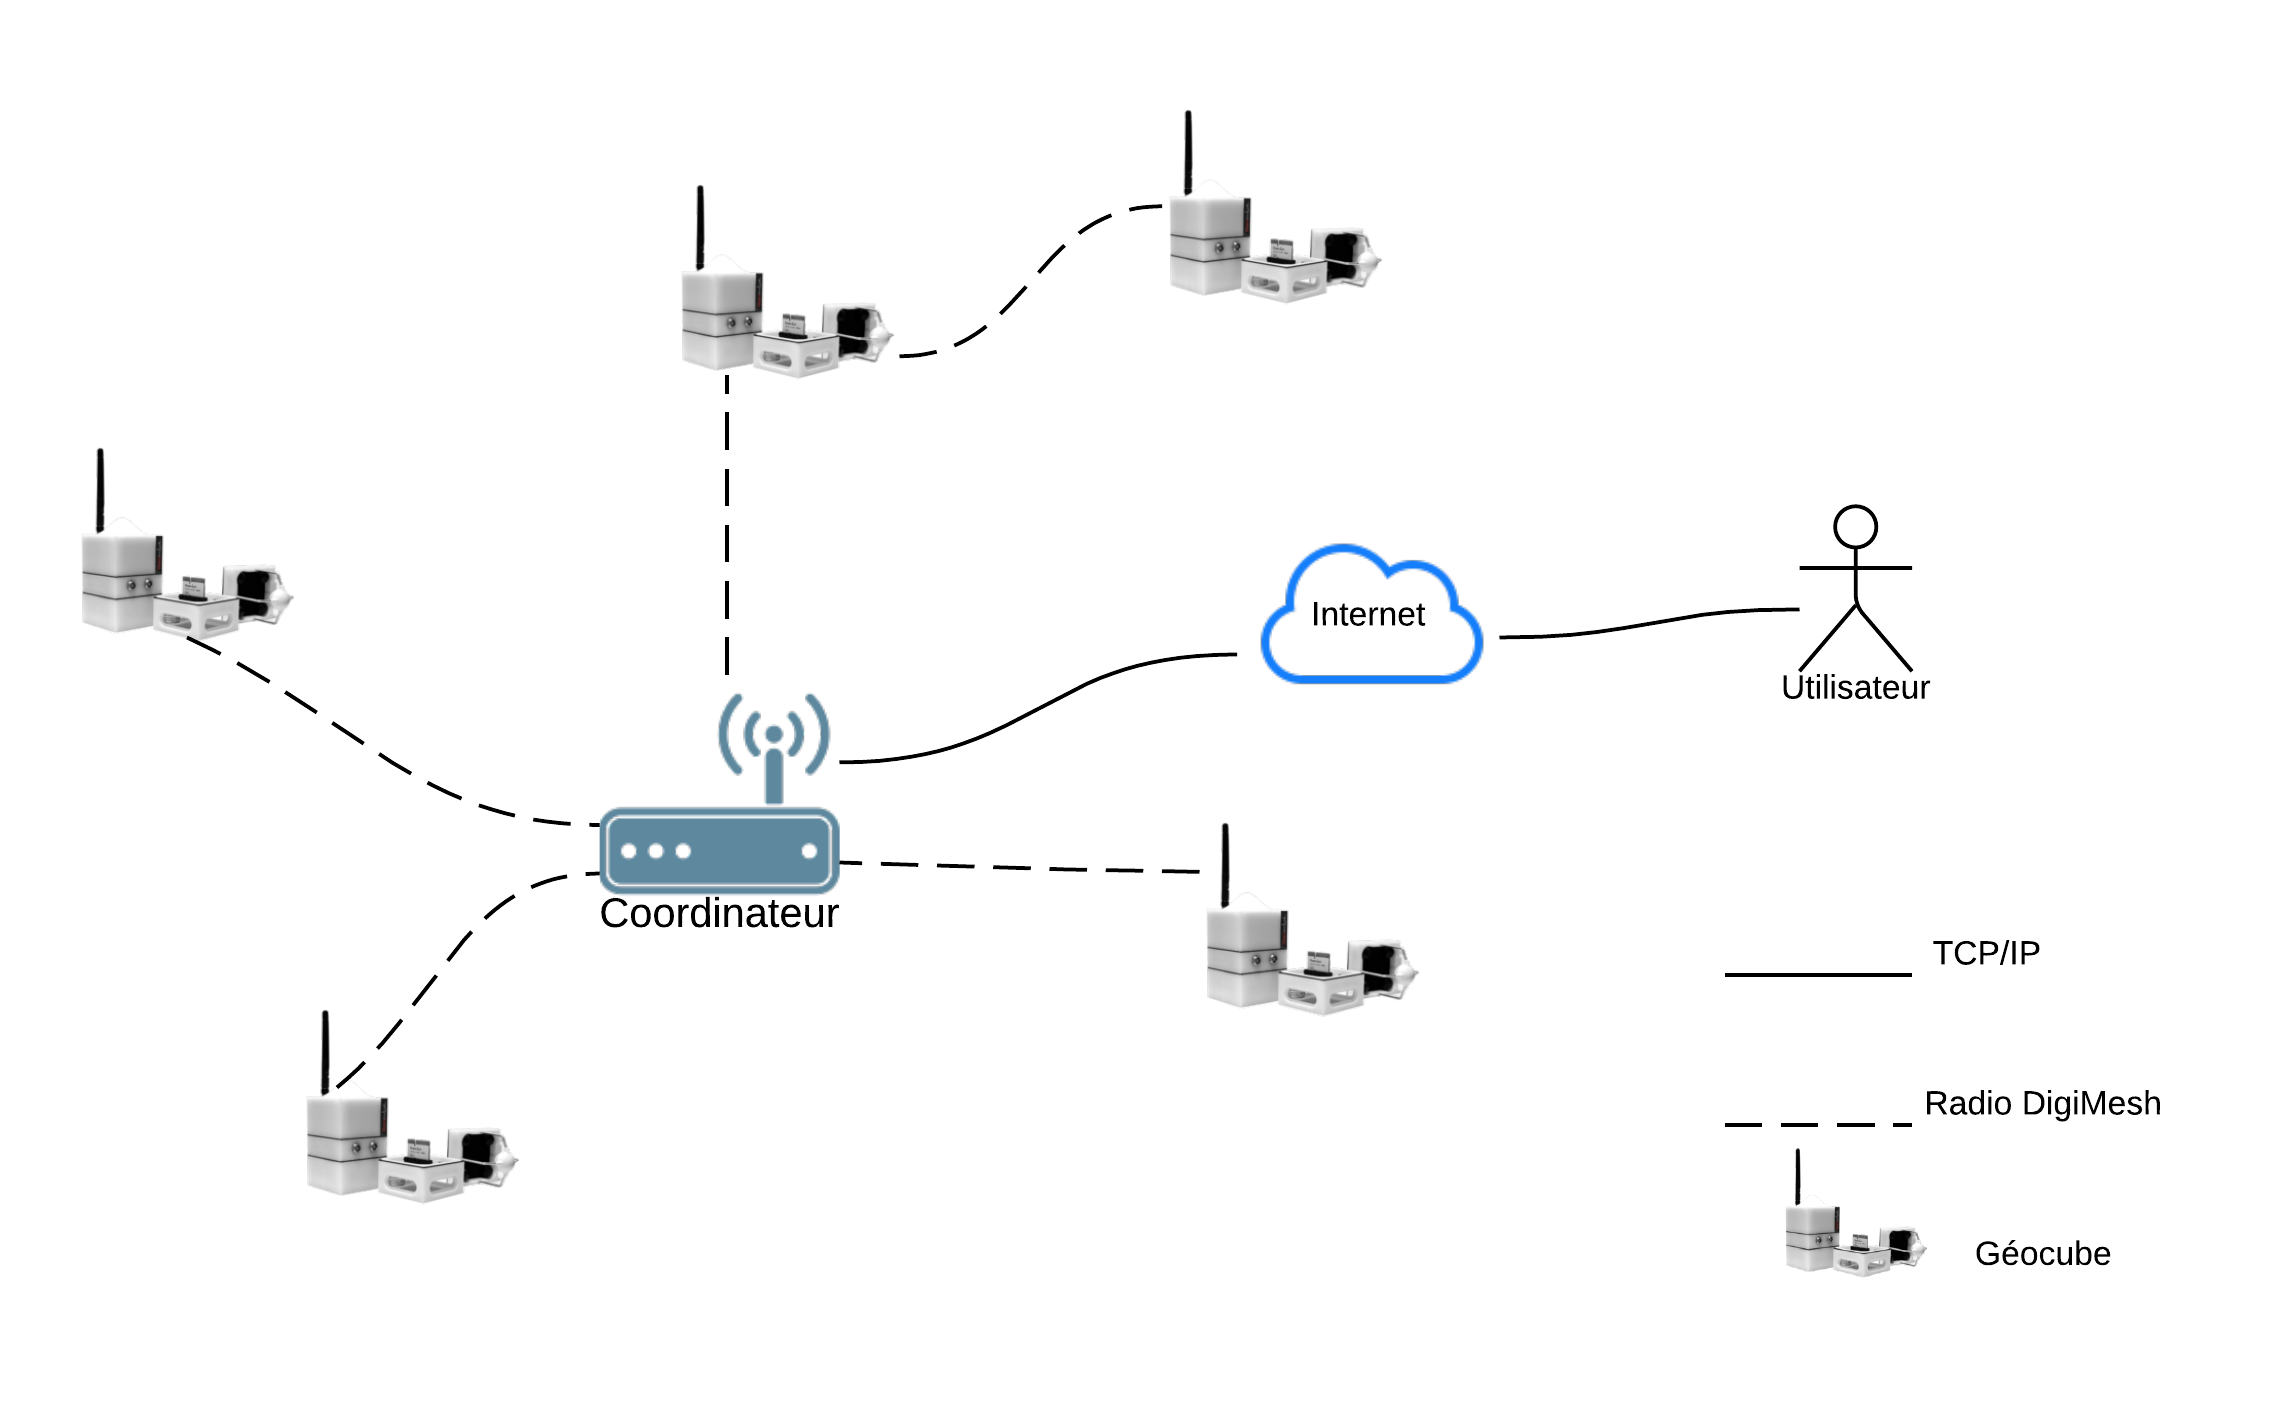
\includegraphics[scale=0.8]{images/fig1.png}
\caption{Un réseau de Géocubes}
\label{fig:geocube_network}
\end{figure}

\section{Les systèmes embarqués et les noyaux temps-réel dur:}
Un système embarqué est par définition: Un système éléctronique et informatique autonome, souvent temps-réel, spécialisé dans une tâche bien précise []. De cette définition on peut ressortir deux éléments clés:
\begin{itemize}
\item Un système embarqué nécessite un développement matériel (électronique) mais aussi logiciel.
\item Un système embarqué a la particularité d'opérer en temps-réel.
\end{itemize}
Le lecteur peut se poser la question légitime: Pourquoi on insiste sur le "temps-réel" dans cette définition? Nos ordinateurs personnels n'opèrent-ils pas en "temps-réel"?. Pour répondre à ces questions et introduire l'importance de ... dans le cas du système Géocube Il faut comprendre que le concept de temps réel en informatique est très relatif et varie d'un métier à un autre: Le temps-réel pour un développeur web est de pouvoir fournir à l'internaute de l'information sous forme de flux, en tolérant les temps de latence qui peuvent résulter parfois des temps d'accès à une base de données ou à la bande passante d'internet. Pour un développeur qui fait de l'informatique pour automobiles et doit, par exemple, développer les couches logicielles relatives à un système d'airbag, Le temps-réel dans ce cas est très strict et la quantification de ce temps latence est primordiale, sinon la vie des gens serait en danger.
\subsection{Les tâches}
Une tâche est le composant principal d'un RTOS. Lorsque vous effectuez plusieurs tâches simultanées sur un ordinateur avec une mémoire vive limitée, vous pouvez remarquer à partir d'un certain ... que vos tâches auront du mal à tourner ... Pour les systèmes d'exploitation en temps-réel, communément connus sous le nom de RTOS (Real Time Operating Systems) La quantification de ce temps de latence est primordiale.

Dans cette perspective, une équipe de chercheurs du LOEMI ont mis au point un RTOS adapté aux tâches qui sont effectuées par un Géocube.

Une liste non exhaustive de ces tâches serait alors:

\begin{itemize}
\item Une tâche GPS qui gère toutes les opérations en relation avec l'acquisition des données GPS:
\item Une tâche Radio qui gère toutes les orpérations relatives à l'envoi et  à la réception des données et des commandes par radio;
\item Une tâche accéléromètre qui gère l'acquisition des données de l'accéleromètre...
\end{itemize}

On note ici qu'à chaque tâche on affecte une priorité. On revient à notre exemple d'airbag pour mieux appréhender cette notion. Imaginons maintenant que dans un RTOS destiné à l'industrie automobile on ne donne pas à la tâche qui gère l'airbag la plus haute priorité. Cela reviendrait à dire qu'à 

\subsection{La communication entre les tâches}

Dans un RTOS généralement, et dans G3OS plus particulièrement, une tâche peut communiquer avec ses semblables ou répondre à des signaux provenant des capteurs, qu'on appelle interruption.

Un signal d'interruption permet à un composant du système embarqué de notifier le micro-contrôleur central de l'arrivée d'un événement qui mérite son attention. Le choix de ces événements se fait souvent en programmant les registres des composants du système. Conventionnellement, le registre qui permet de choisir les événements déclencheurs d'interruptions s'appelle le registre principal des interruptions (Main Interrupt Register).

La communication entre les tâches s'effectue par plusieurs méthodes. La principale connue est la queue de messages. Ce mécanisme permet à une tâche de communiquer avec les autres en envoyant des messages. Un exemple typique serait alors: une tâche qui s'occupe de l'acquisition des données d'une puce GPS. Dès qu'une nouvelle trame de données est disponible, Cette tâche envoie  et une autre du traitement de ces données, Dans ce cas la première tâche envoie à la deuxième les données acquises à travers la que

\begin{figure}[h!]
\centering
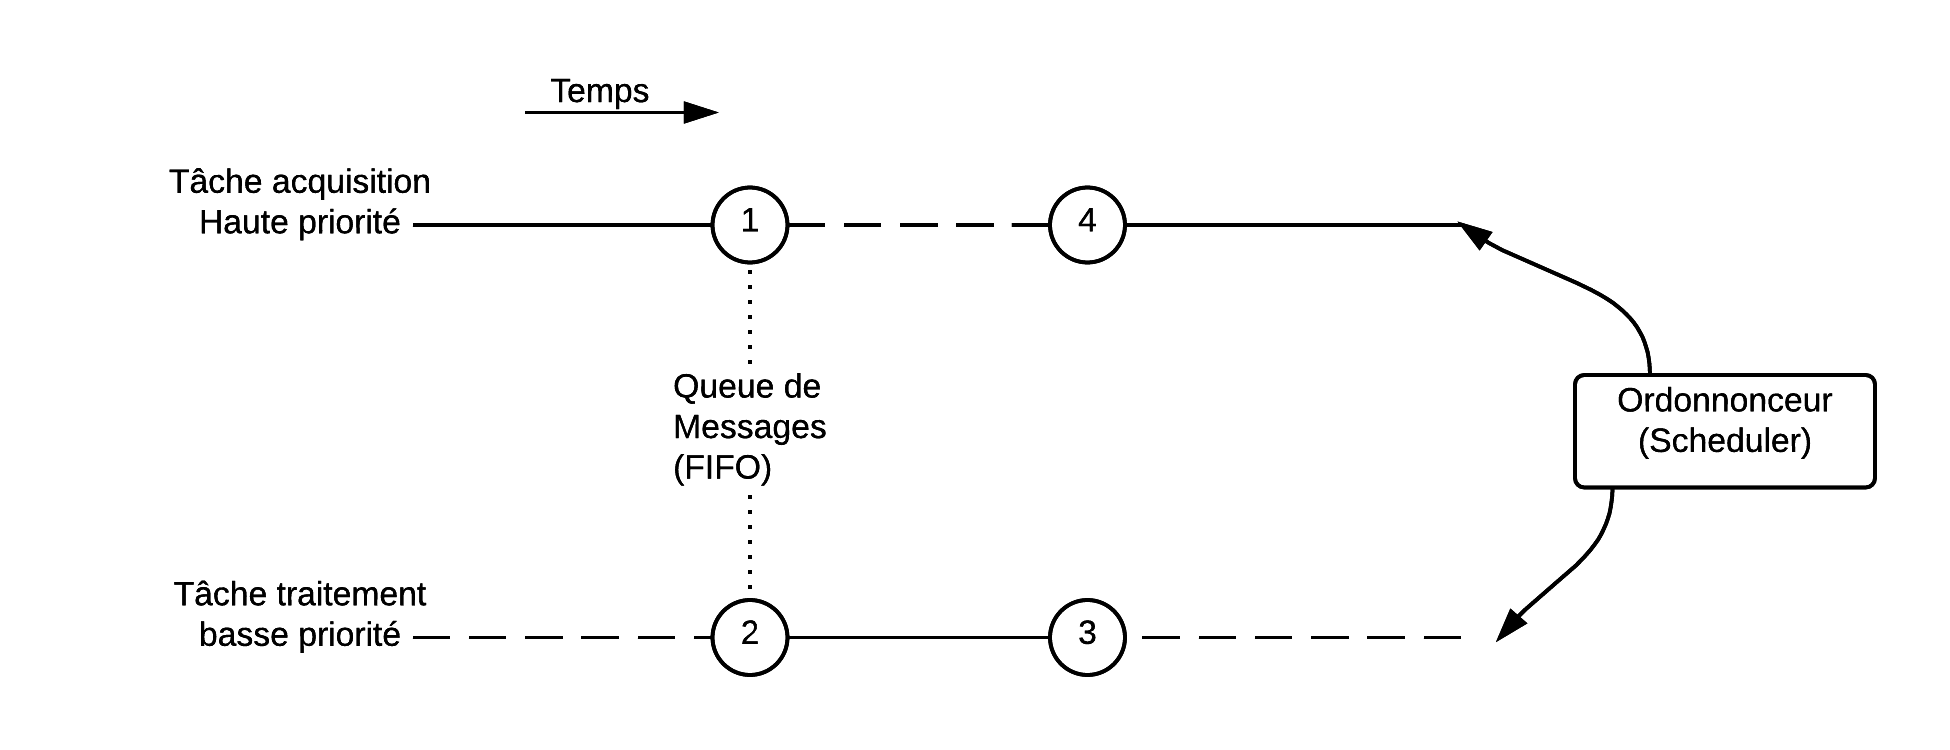
\includegraphics[scale=1]{images/fig2.png}
\caption{Exemple multi tâches}
\label{fig:multitask_ex}
\end{figure}

\section{La communication en champs proche (NFC)}
La communication en champs proche est un ensemble de protocoles permettant d'établir une connexion radio entre deux dispositifs avec une distance ne dépassant pas 4cm. Aujourd'hui, on compte des millions d'objets connectés contenant la technologie NFC(cartes bancaires, smartphone, arrêts de bus, smartwatch...). L'interopérabilité entre les différentes puces équipant ces objets a poussé les constructeurs à mettre en place un certain nombre de normes régissant la fabrication, la programmation et l'utilisation de cette technologie.

La guerre des normes a fait converger les constructeurs vers l'ISO/IEC 14443. Cette norme encapsule en elle même quatre sous normes:

\begin{itemize}
\item ISO/IEC 14443-1: Description des couches physiques
\item ISO/IEC 14443-2: 
\item ISO/IEC 14443-3:
\item ISO/IEC 14443-4: 
\end{itemize}

\subsection{couches matérielles:}
La conception des couches matérielles d'un circuit NFC doit respecter les recommandations de l'ISO/IEC 14443-1 et une partie de l'ISO/IEC 14443-2 pour garantir l'interopérabilité avec les autres dispositifs disponibles sur le marché. Un circuit NFC typique est composé de 3 parties principales:
\begin{itemize}
\item Une antenne: Selon les spécifications de la dite norme les dimensions de l'antenne ne doivent pas excéder 86mm x 54mm x 3mm.
\item Une capacité adaptée pour garantir une raisonnance du circuit sur la fréquence 13.56Mhz;
\item Le PICC
\end{itemize}
\subsection{couches logicielles:}


\section{Les infrastructures de production des logiciels}
La conception et le développement des solutions logiciels dans un milieu industriel nécessite des infrastructures permettant d'automatiser un certain nombre de tâches qui, ensemble, forment ce qui est communément connu sous le nom de pipeline de production logicielle.

Cette chaîne de production est itérative, Elle favorise les cycles courts pour délivrer au client un produit évolutif et s'adaptant à ses besoins. Dans la Figure... on présente les principales étapes de cette chaîne.

Comme montré dans la Figure.... Une pipeline de production logicielle a un certain nombre d'acteurs externes humains qui garantissent son alimentation en versions(1) et en tickets(2). On définit alors ces acteurs comme suit:

\begin{itemize}
\item Développeur: s'occupe de la conception et le développement des solutions informatiques en réponse aux besoins des clients exp.. dans le gestionnaire des bugs. Son travail permet d'alimenter le gestionnaire de versions.
\item Product owner: terme emprunté à la méthode Scrum. Il est l'interlocuteur unique des clients et permet de traduire leurs besoins en tickets(Gestionnaire de tickets)
\item Testeur: 
\end{itemize}
En plus de ces acteurs humains une infrastructure de production logicielle contient des composants logiciels pour automatiser un certain nombre de tâches:
\begin{itemize}
\item Gestionnaire de bugs: Comme son nom l'indique ce composant est un outil de communication et de traçabilité permettant de suivre l'évolution de la réponse du développeur au besoin du client et à la correction des bugs.
\item Gestionnaire de versions: Cet outil est un classique de la gestion des projets informatiques, il permet, entre autres, aux développeurs de collaborer sur le même code source sans que cela n'affecte  d'archiver tous les changements effectués sur un code source. Par souci de traçabilité, un gestionnaire de version est indispensable dans un projet informatique même s'il n y a qu'un développeur.
\item Intégration continue
\end{itemize}


\evenchapter[Conception et développement des couches logicielles et matérielles relatives à la norme NFC ISO14443 et de l'IHM Android dédiée]{Conception et développement des couches logicielles et matérielles relatives à la norme NFC ISO14443 et de l'IHM Android dédiée}

\section{Analyse du besoin:}
Dans le but de simplifier au maximum la mécanique et d’assurer au mieux l’étanchéité de celle-ci, il est prévu dans la version industrielle du geocube de n’utiliser ni interrupteur On/Off ni connecteur permettant de communiquer avec le geocube par un lien filaire. La seule possibilité de lien se fera par la radio, dont le débit est trop faible pour assurer des transfert de fichiers de données.

Solution :

Nous proposons donc d’inclure dans le geocube la fonctionnalité NFC. Elle devra pouvoir déclencher l’allumage ou au moins le réveil de sommeil profond du processeur du geocube, ainsi que son extinction. Elle devra aussi pouvoir servir de lien de communication avec le logiciel de commande du geocube pour permettre la configuration et le test de bon fonctionnement du geocube par exemple lors de son installation. Enfin, elle permettra le déchargement et le chargement de fichiers depuis et vers la carte µSD.
Le stage se déroulera en plusieurs phases :

- Identification du chipset NFC à utiliser. Il y en a un déjà dans le design actuel, il faudra vérifier si ses performances sont suffisantes.

- Modification ébventuelles de la carte du geocube pour intégrer le circuit choisi et assurer les fonctionnalités demandées.

- Test du chipset choisi.

- Réalisation des couches logicielles interface dans G3OS

- Réalisation d’une appli dédiée sous Android pour l’IHM

\section{Conception de la solution:}
\subsection{Choix de la puce NFC:}
Le choix d'une puce NFC s'est basé sur une webographie effectuée sur les sites des constructeurs pour trouver la puce la plus adaptée à la description du besoin du commanditaire. Une puce NFC doit répondre au mieux à ce besoin tout en encapsulant le maximum de fonctionnalités des 3 derniers niveaux (2, 3 et 4) de la norme ISO-14443. Cette norme garantie l'interaction avec les dispositifs utilisant le système exploitation Android.

Après une première analyse des caractéristiques de quelques dix puces sélectionnées, On ne garde pour la suite que les trois citées dans le Tableau ci-dessous. La plupart des puces disponibles dans le marché et qui sont interfaçables avec un micro-contrôleur\footnote{La plupart des puces sont stand-alone et programmable une fois.}.
\begin{figure}
\begin{center}
\begin{tabular}{|c|c|c|c|c|c|c|c|}
\hline
Référence & Constructeur & Prix(\$) & Débit(kbps) & ISO 14443 & Interface & T° & RAM\\ \hline
TRF7970A & TI & 6.98 & 424 & 3 & SPI-Paral & -40°-110° & NC\\
RF430CL330H & TI & 1.74 & 848 & 3 & SPI-I2C & -40°-85° & 3KO\\
AS3953 & AMS & 1.09 & 848 & 3 & SPI & -40°-85° & NC\\
PN533 & NXP & NC & 848 & 3 & USB2 & -40°-125° & 1KO\\
\hline
\end{tabular}
\end{center}
\caption{Tableau comparatif des puces NFC présélectionnées.}
\end{figure}

On remarque qu'aucun constructeur ne propose des puces compatibles avec le 4ème niveau de la norme ISO/IEC 14443. L'utilisation de cette norme est indipensable pour pouvoir communiquer avec un dispositif Android\footnote{Android n'accepte pas les protocoles propriétaires pour la communication en champ proche. Que les protocoles certifiés par l'ISO/IEC}. Un travail serait alors à effectuer pour programmer le niveau manquant de la dite norme dans le micro-contrôleur.

Une puce existe déjà dans la version actuelle du Géocube. C'est l'AS3953, Le maintien de cette puce permettra de gagner:
\begin{itemize}
\item en temps de développement matériel.
\item en prix: c'est la moins cher de sa catégorie.
\item ultra basse consommation électrique\footnote{Ce qui est crucial pour le Géocube} Dans plusieurs cas d'utilisation la puce s'alimente de l'énergie émise par le smartphone.
\end{itemize}
Pour ces raison le choix de l'AS3953 a été maintenu pour le Géocube.

\subsection{Conception et expérimentation de l'antenne:}

Les prototypes des antennes NFC sont généralement conçus d'une manière empirique. Pour cela, Il existe plusieurs méthodes expérimentales conventionnelles. Mais avant de présenter les expériences réalisées. Il faut comprendre qu'un circuit NFC typique peut être assimilé à un circuit de type RLC. L'équivalent électrique d'une puce NFC et son antenne pourrait être assimilé au circuit de la Figure\ref{fig:nfcandantenna}.

\begin{figure}[h!]
\centering
\label{fig:nfcandantenna}
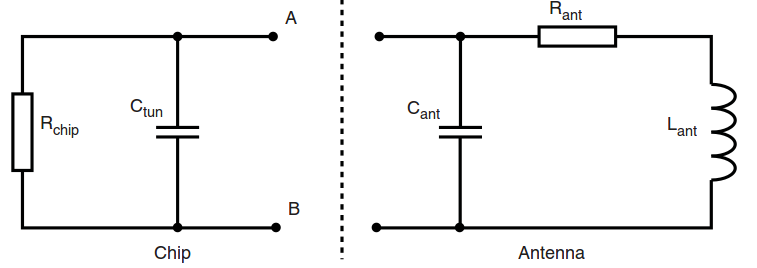
\includegraphics[scale=0.5]{images/chipANDantenna.png}
\caption{Circuit électrique équivalent d'une puce NFC et et son antenne}
\end{figure}
l'antenne est un fil conducteur, son équivalent électrique est la résistance $R_{ant}$. Elle a aussi une inductance qu'on note $L_{ant}$ et une capacité parasite $C_{ant}$. Alors que $R_{chip}$, $C_{tun}$ désignent respectivement la résistance et la capacité introduits par la puce NFC.

La Figure\ref{fig:nfcandantenna} est un schéma simplifié du circuit électronique que présente une antenne et une puce NFC puisqu'il ne prend pas en compte les connexions filaires entre les deux. Un schéma plus global peut se présenter comme dans la Figure\ref{fig:completeeq} lorsque l'antenne ajoute une résistance en série et dans la Figure\ref{fig:completeeq2} lorsque qu'elle inclut une résistance en parallèle.

\begin{figure}[h!]
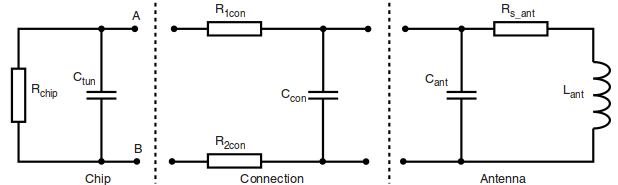
\includegraphics[scale=0.7]{images/chipANDantennaANDconn.png}
\label{fig:completeeq}
\caption{Circuit électrique équivalent d'une puce NFC, une antenne avec une résistance en série et les liaisons filaires entre les deux}
\end{figure}

\begin{figure}[h!]
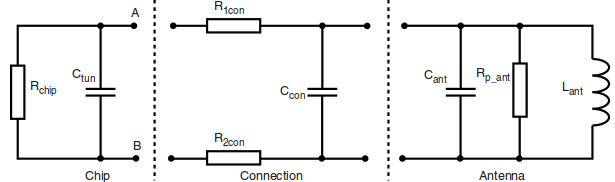
\includegraphics[scale=0.7]{images/withPARA.png}
\label{fig:completeeq2}
\caption{Circuit électrique équivalent d'une puce NFC, une antenne avec une résistance en parallèle et les liaisons filaires entre les deux}
\end{figure}
\begin{itemize}
\item $R_{con}$: La résistance équivalente parasite générée par les fils de connexion entre la puce NFC et l'antenne.
\item $C_{con}$: La capacité équivalente parasite générée par les fils de connexion entre la puce NFC et l'antenne.
\item $R_{s-ant}$: La résistance en série de l'antenne.
\item $R_{p-ant}$: La résistance en parallèle de l'antenne.
\end{itemize}
En calculant la résistance et la capacité équivalentes on obtient la Figure\ref{fig:circuiteq}. $R_{eq}$ est calculée comme suit:

\begin{figure}
\centering
\label{fig:circuiteq}
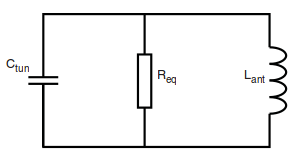
\includegraphics[scale=0.6]{images/circuiteq.png}
\caption{Circuit simplifié d'une puce NFC, une antenne et les connexions filaires entre les deux}
\end{figure}

$$R_{eq}=\frac{R_{chip}\times R_{p-ant}}{R_{chip}+R_{p-ant}}$$

alors que:

$$R_{p-ant}=R_{s-ant}\times(1+(\frac{L_{ant}\times\omega}{R_{s-ant}})^2)$$

La fréquence de raisonnance $f_0$ d'un circuit LC parallèle peut être calculée en utilisant cette formule:

$$f_0=\frac{1}{2\pi\sqrt{L_{ant}.C_{tun}}}$$

L'inductance de l'antenne à la raisonnance peut être exprimée comme suit:
$$L_{ant}=\frac{1}{(2\pi.f_0)^2.C_{tun}}$$

Dans la plupart des cas on dispose de l'inductance $L_{ant}$ dans les datasheets des antennes. La grandeur qui reste à déterminer est alors $C_{tun}$. Comme nous avons vu précédemment:

$$C_{tun}=C_{chip}+C_{conn}+C_{ant}$$

Les valeurs de $C_{ant}$ et $C_{chip}$ sont généralement disponibles dans les datasheets de l'antenne et de la puce NFC. Théoriquement, La seule grandeur qui reste à déterminer est $C_{conn}$:

$$C_{conn}=C_{tun}-C_{chip}-C_{ant}$$

Malheureusement, ce n'est pas toujours le cas\footnote{Comme c'est le cas pour le Géocube} le circuit imprimé sur lequel vient s'ajouter l'antenne NFC peut modifier l'inductance de l'antenne d'une manière (pseudo-)aléatoire et dépendante des composants rayonnants du circuit, en plus du plan de masse que peut présenter ce dernier. Un mode opératoire itératif qui consiste à faire varier la capacité $C_{conn}$ jusqu'à ce que la fréquence de raisonnance du circuit se stabilise autour de 13.56Mhz serait alors de.

Pour cela nous avons conçu l'expérimentation schématisée sur la Figure\ref{experience} Le but est alors de mesurer pour chaque itération(et donc pour chaque valeur de capacité) la fréquence de raisonnance du circuit à une antenne qui émet à 13.56Mhz\footnote{Ce qui simule l'antenne NFC d'un smartphone}, et ceci jusqu'à trouver la capacité pour laquelle le circuit: Géocube+antenne raisonne à 13.56Mhz. Un GBF(Générateur de Basses fréquences) réglé sur 13.56Mhz et lié à une antenne simule un smartphone avec son antenne NFC. Le but serait alors de mesurer à chaque itération, à l'aide d'un oscilloscope.

\begin{figure}[h!]
\centering
\label{experience}
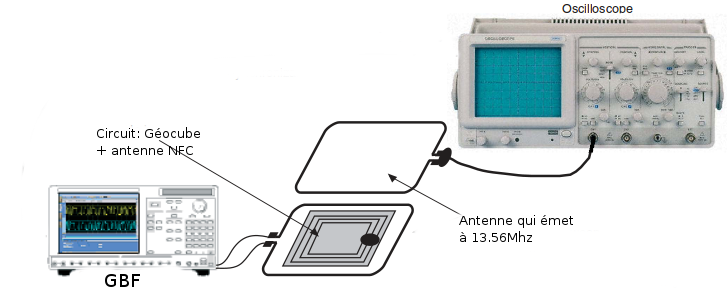
\includegraphics[scale=0.55]{images/gbfoscillo.png}
\caption{Expérimentation réalisée pour calibrer l'antenne NFC du Géocube}
\end{figure}
Les antennes testées sont des circuits éléctroniques imprimés que nous avons conçus spécialement pour le Géocube
Cette expérimentation a permit de choisir une capacité pour les modèles d'antennes....

\subsection{Conception des couches logicielles}
La puce NFC retenu n'inclut pas le niveau 4 de la norme ISO/IEC 14443. Ce niveau est indispensable pour pouvoir communiquer avec d'autres dispositifs NFC et spécialement les smartphones utilisant un système d'exploitation Android.

\evenchapter[Conception, développement et déploiement d'un système de mise à jour automatique destinée au système Géocube:]{Conception, développement et déploiement d'un système de mise à jour automatique destinée au système Géocube:}
\textit{ Dans ce chapitre plusieurs diagrammes UML(Unified Modelling Language) sont utilisés pour simplifier la conception du système de mise à jour au lecteur. Pour plus d'informations sur le langage voir []. Le système de mise à jour développé fut baptisé Sharokey}
\section{Étude du besoin:}
Le besoin se fait ressentir de plus en plus au sein de la société Kylia de disposer d'un système permettant aux clients qui ont acheté un système Géocube  d'eefectuer des mises à jour automatiques et de profiter ainsi des améliorations éventuelles qui seront amenées aux couches logicielles des produit sans pour autant procéder à un rappel de celui ci.

En plus du de la gestion des mises à jour, ce système doit être au coeur de plusieurs métiers, permettant de coordonner le travail entre le développeur, l'administrateur système, l'opérateur commercial et les clients désirant profiter des dernières améliorations portées sur les couches logicielles.

\begin{figure}[h!]
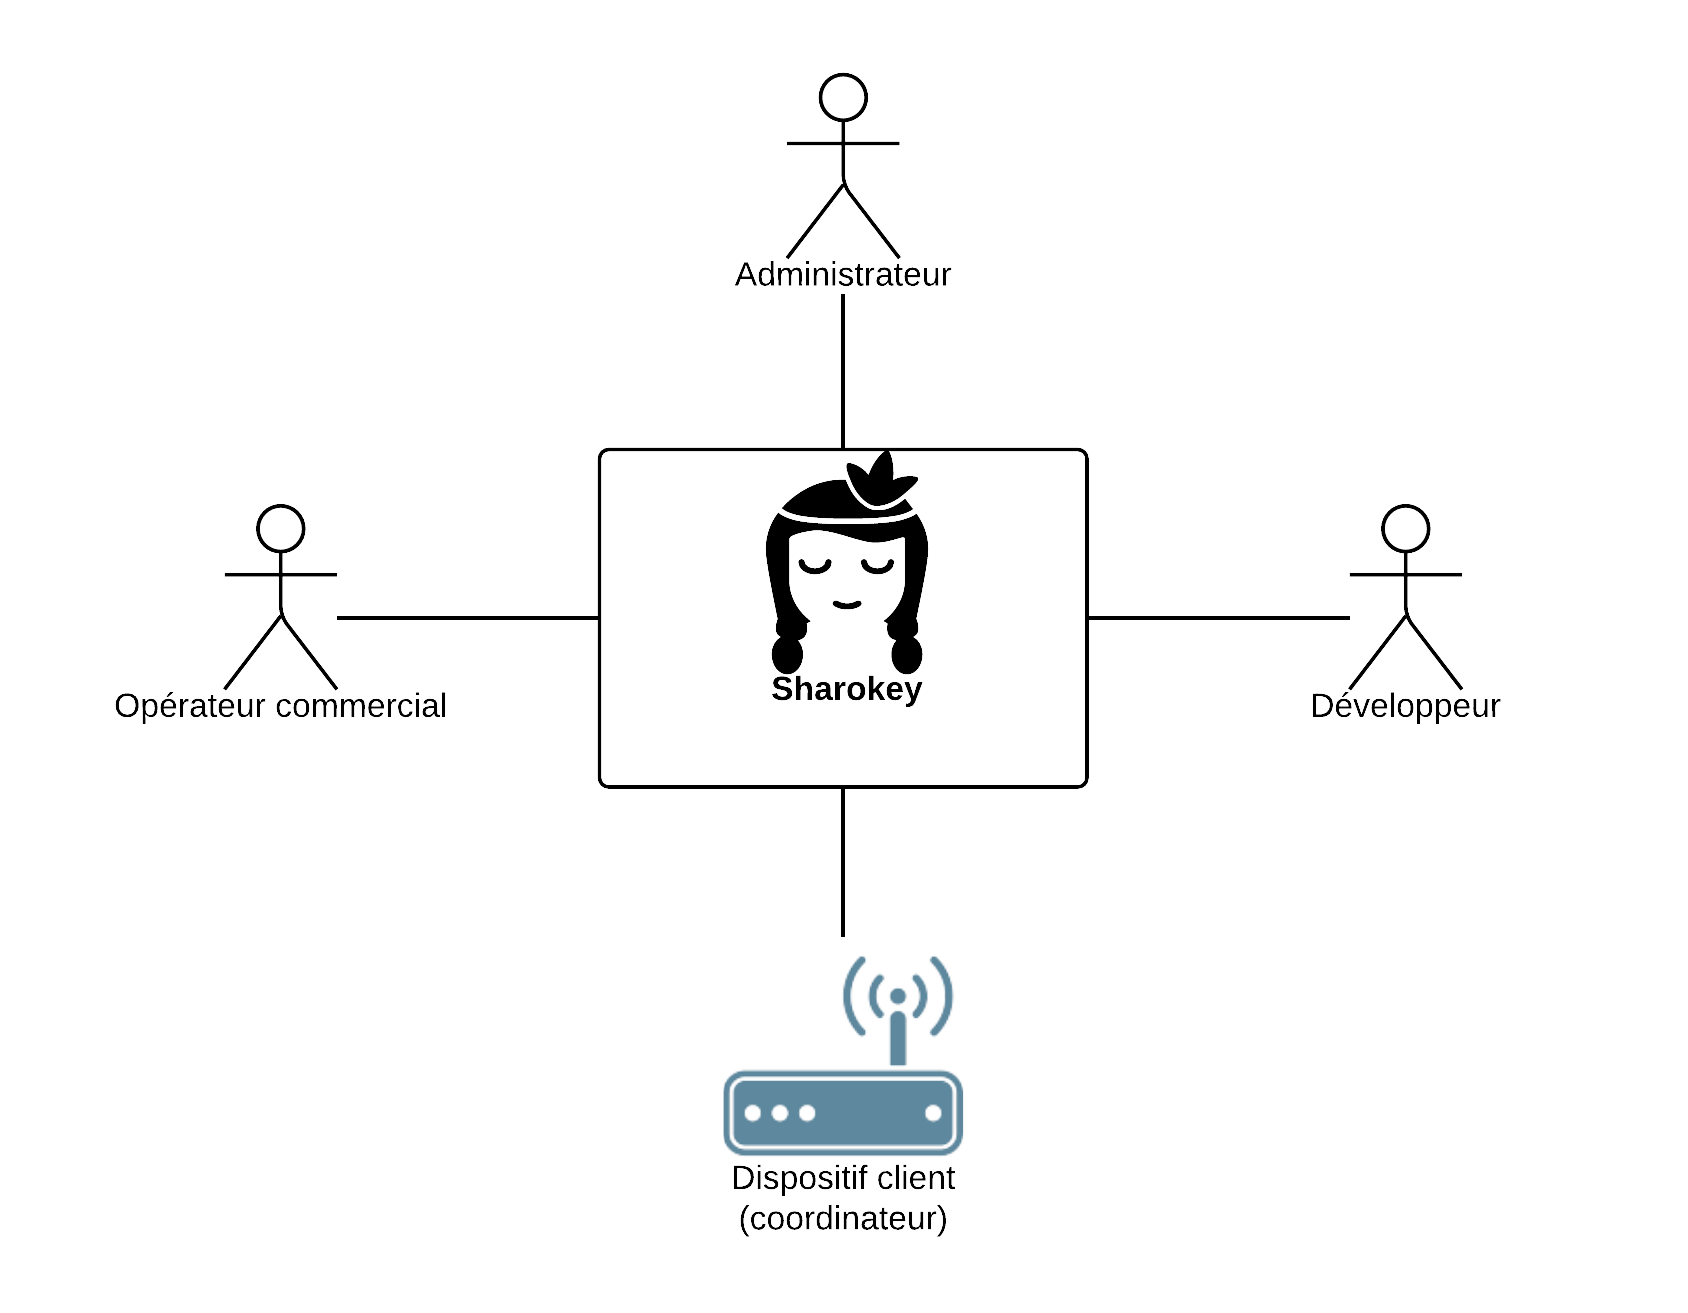
\includegraphics[scale=0.9]{images/context_general.png}
\label{fig:context_statique}
\centering
\caption{Diagramme de contexte statique}
\end{figure}

De la Figure\ref{fig:context_statique} on définit les acteurs suivants:
\begin{itemize}
\item Opérateur commercial: Personne qui procède à la vente des systèmes Géocubes et des licences de mise à jour. Une licence a un date de début et une date de fin. Elle détermine la période ((pour laquelle)) le client à le droit de profiter du support logiciel à travers la mise à jour de son dispositif.
\item Développeur: Personne responsable de l'alimentation continue du système en versions.
\item Administrateur: Personne responsable de l'administration et la supervision du système de mise à jour.
\item Coordinateur: Dispositif client destiné à être mis à jour.
\end{itemize}

Ce système doit en plus présenter les particularités suivantes:
\begin{itemize}
\item La supervision et l'administration du système doit être simplifiée à travers des interfaces homme-machine.
\item 
\item Les logs du système doivent être expressifs et facilement accessible par l'administrateur.
\item Les requêtes du client et les réponses du serveur doivent être sécurisées.

\end{itemize}

\section{Conception statique}
La Figure\ref{fig:use_case} résume les cas d'utilisation de Sharokey.

\begin{figure}[h!]
\centering
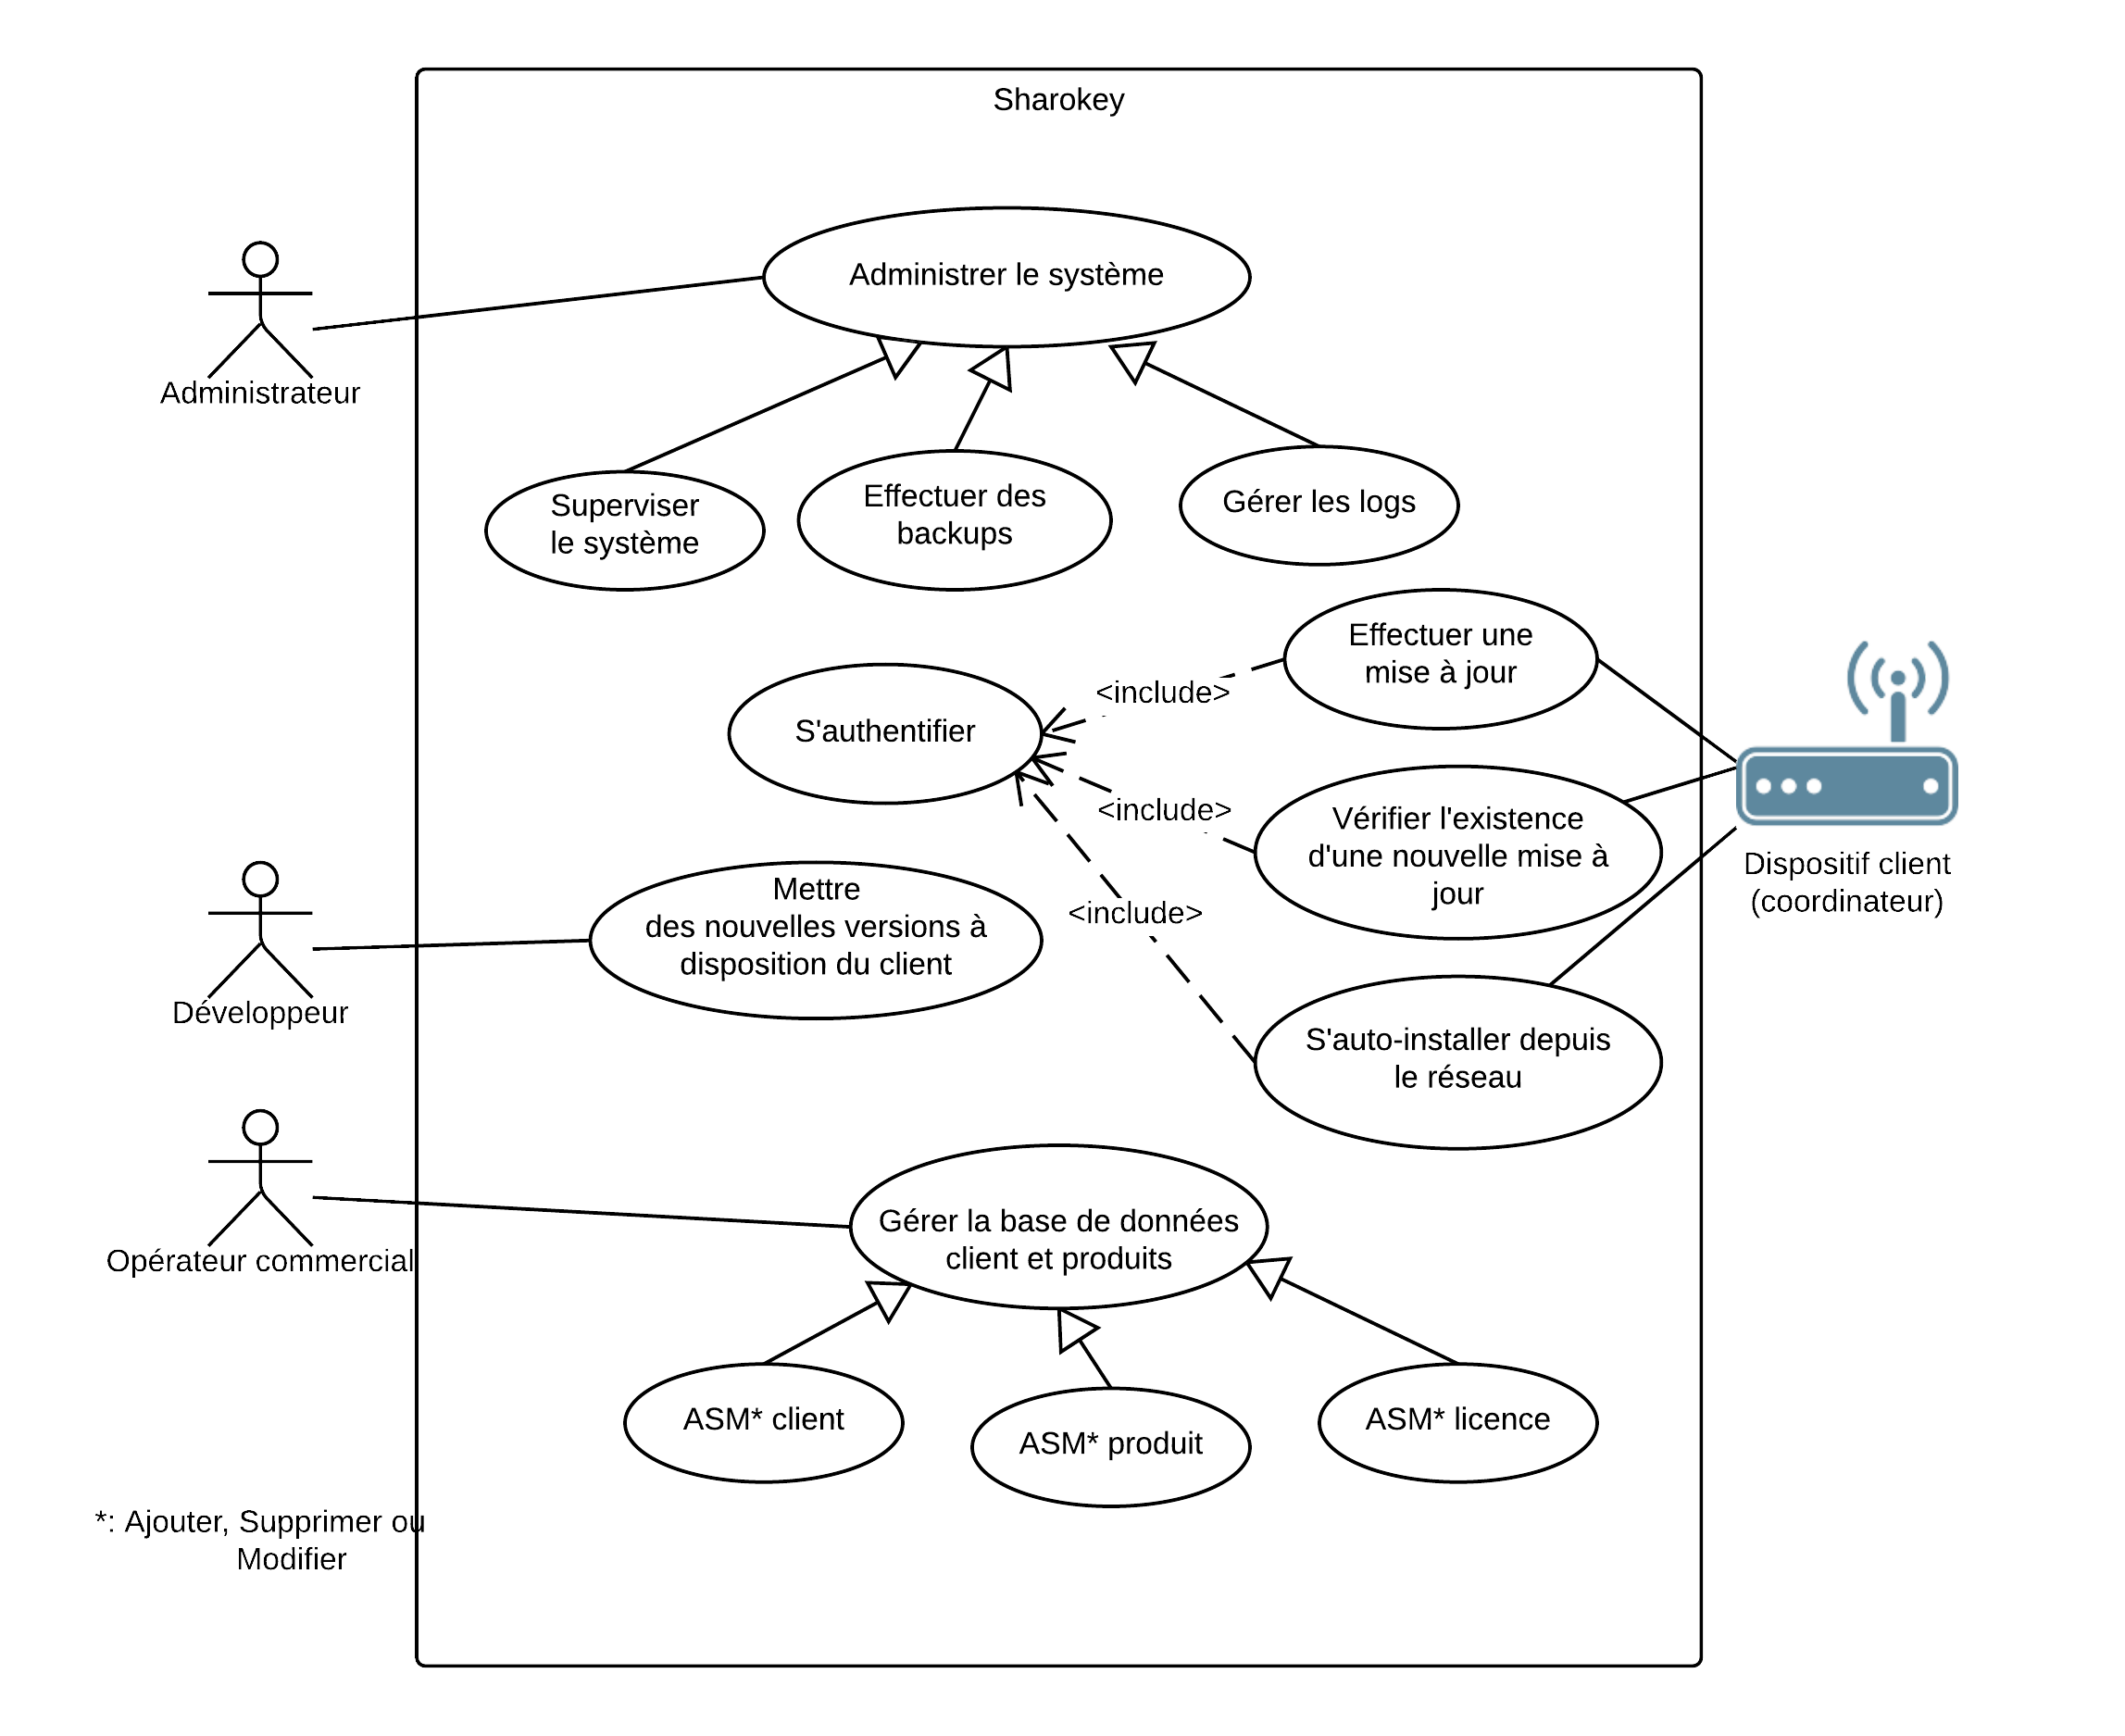
\includegraphics[scale=1]{images/use_case_sharokey.png}
\label{fig:use_case}
\caption{Diagramme UML des cas d'utilisation de Sharokey}
\end{figure}

La modélisation de la base de donnée est présentée dans la Figure\ref{fig:mpd}. On définit alors les entités suivantes:
\begin{itemize}
\item client: Personne physique qui effectue la commande d'un produit, elle est identifiée par IDC (clef primaire ID Client). Cette personne peut appartenir à une institution (entreprise ou organisme étatique), Les autres champs de la table servent à identifier les informations nécessaires au contact: Nom, Prénom, Téléphone, E-mail et un commentaire qui est laissé au soins de l'opérateur commercial.
\item product: C'est le coordinateur qui est destiné à recevoir les mises à jour. Il est identifié par son Part-Number (IDP). On lui attribue en plus un nom qui est généralement celui de la marque du fabriquant.
\item license: Entité qui établie la relation entre la table product et la table client, en utilisant des clés étrangères vers leurs identifiants. Elle attribue à chaque client une licence de mises à jour sur un produit pour une durée comprise entre une date de début (start date) et une date de fin (end date).
\item software: C'est la table qui contient toutes les mises avec les numéros de versions correspondants. Elle contient une clef étrangère vers la table product, puisque chaque mise à jour est destinée à un produit particulier. chaque mise à jour est identifiée par une version majeure, une version mineure et une version de patchs. La version 1.0.5 correspond alors à la version majeure 1, la version mineure 0 et la version de patchs 5. En plus, chaque mise à jour a un type qui peut être soit V (pour version), ou P pour (patch). La différence réside dans la pertinence des améliorations portées.
\item Les triggers: Deux triggers pour écouter les événements des tables: client et product.
\end{itemize}

\begin{figure}
\centering
\label{fig:mpd}
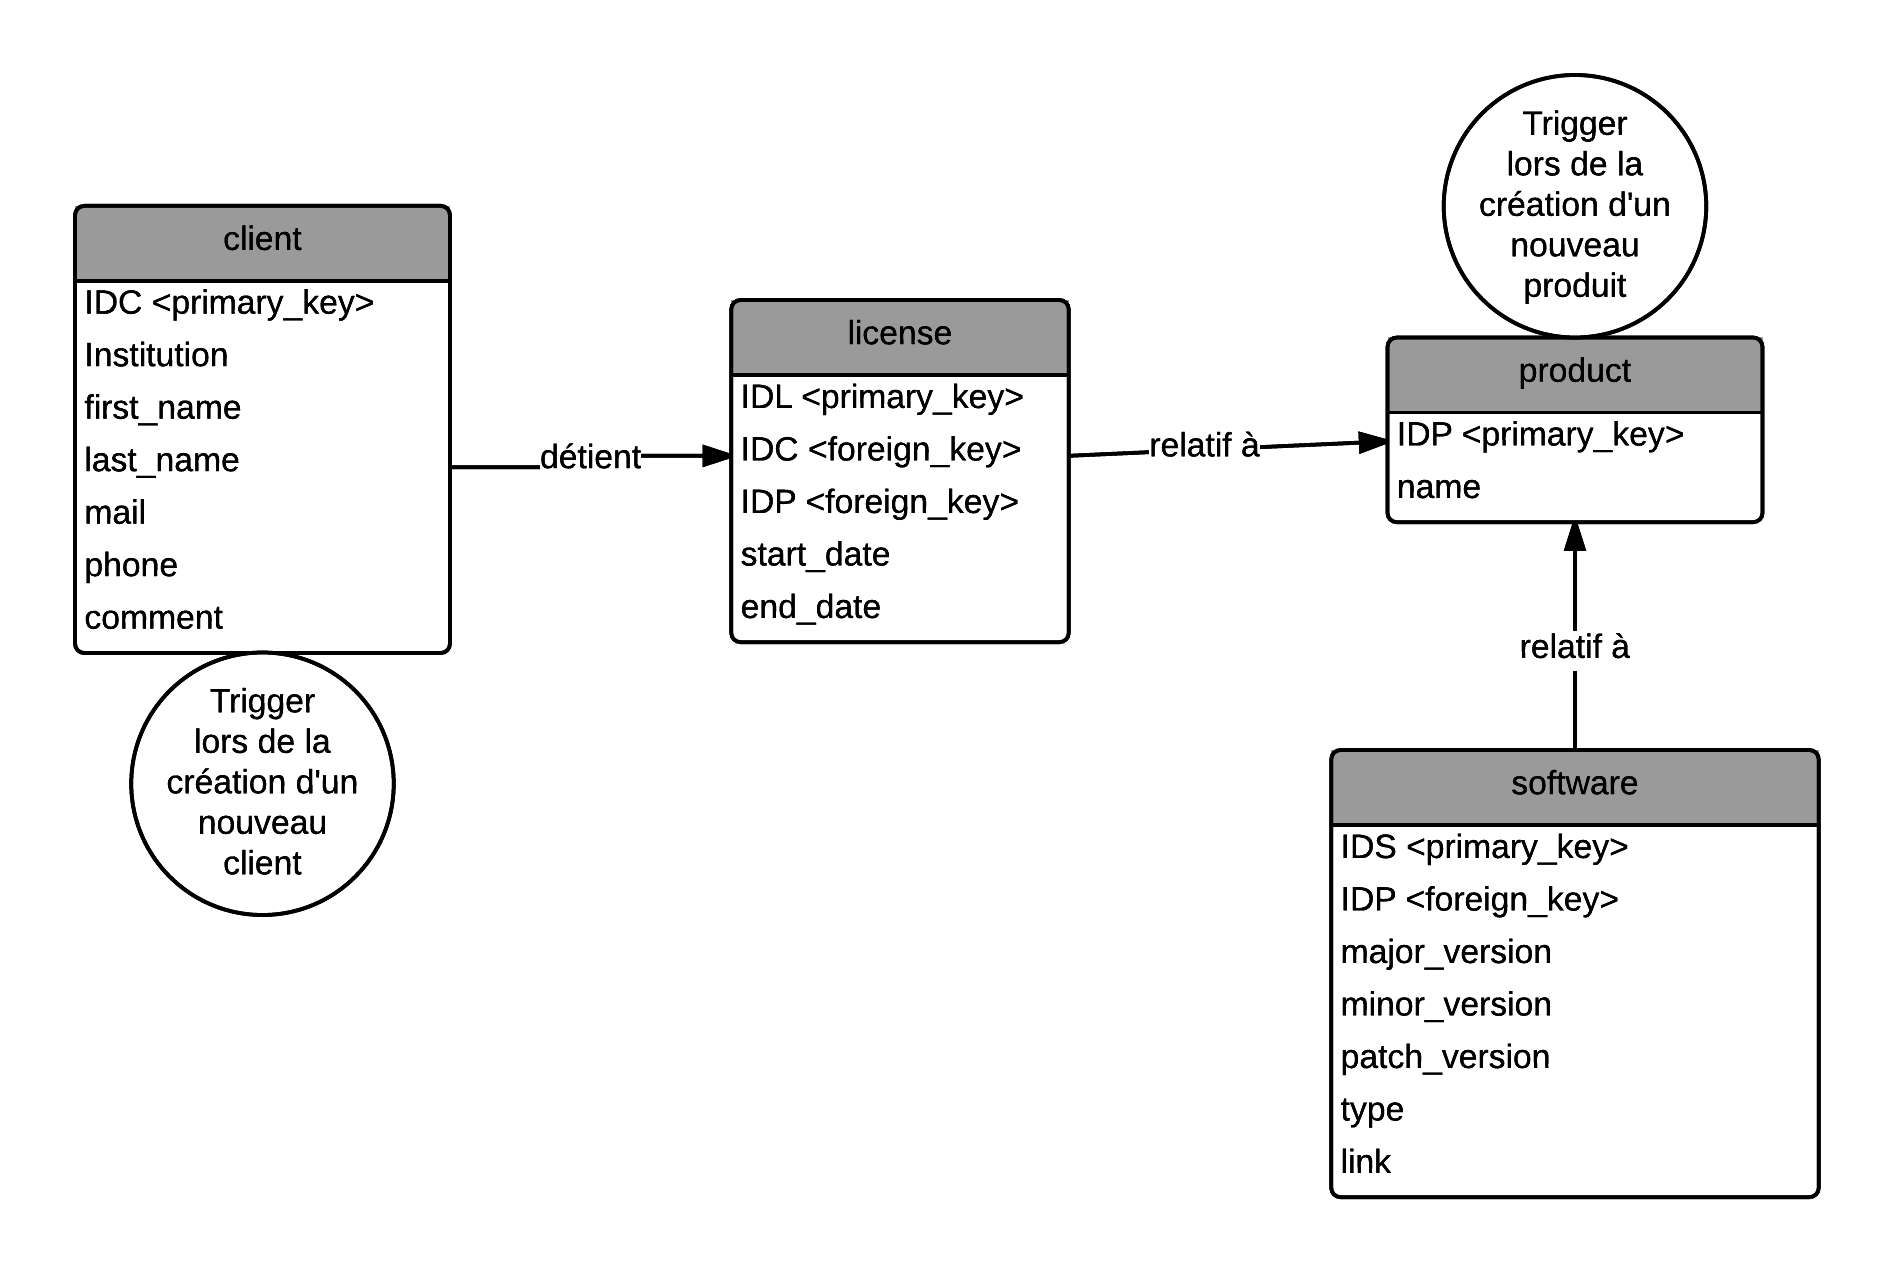
\includegraphics[scale=0.85]{images/MPD_sharokey.png}
\caption{MDP (Modèle Physique des Données) de la base de données Sharokey}
\end{figure}
\subsection{Format des mises à jour}

Une mise à jour est un script auto-extractible fabriqué en utilisant le programme Makeself. Un format de paquets a été conçu pour simplifier et automatiser la création des scripts de mise à jour. Ce format a un point d'entrée qu'on nomme "go.sh" et un répertoire de scripts et de données baptisé "installerScripts". go.sh est un script shell qui execute les scripts contenus dans installerScripts. la fabrication d'un éxecutable auto-extractible à partir de ces éléments en utilisant Makeself permet d'ajouter un mécanisme de vérification de l'intégrité du paquet de mise à jour avec une somme MD5.

\subsection{Architecture logicielle}
Sharokey est une solution informatique légère de mise à jour automatique pour les solutions informatiques propriétaires basés sur un système d'exploitation GNU/Linux et nécessitant une licence ou une autorisation pour faire les mises à jour. Il est basé sur une architecture client-serveur. Le client est codé entièrement en Shell pour garantir une portabilité sur toutes les distributions GNU/Linux et sur une grande panoplie d'architectures matérielles: Intel, ARM, MIPS, ... Le serveur est écrit en NodeJS. Ce choix garantie se portabilité sur les serveurs utilisant des OS type Windows ou GNU/Linux. Toute fois, il est fortement conseillé d'utiliser GNU/Linux. Les tests effectués jusqu'à ce jour n'ont porté que sur ce type d'OS.

\subsubsection{Client:}
Comme schématisé dans la Figure, La partie client est contituée d'un ensemble de paquets Kylia dont nous présentons les fonctionnalités ci-dessous:
\begin{itemize}
\item checker.kyl: Ce paquet renvoie trois codes possibles 0, 1 ou 2. 0 si le dispositif client arrive à se connecter au serveur mais aucune nouvelle mise à jour n'est disponible. 1 si le dispositif client arrive à se connecter au serveur et il y a une nouvelle mise à jour a effectué. 2 si le dispositif client n'arrive pas à se connecter à internet\footnote{Le code retour 2 est important pour le coordinateur des Géocubes, puisque ce dernier est dépendant d'internet. Ce code retour permet d'informer le client d'un souci de réseau}.
\item update.kyl: Ce paquet télécharge et éxécute les mises à jour, il change ensuite le numéro de la version courante dans le dispositif client pour l'adapter à celle du serveur.
\item zeus.kyl: Ce script a pour but d'automatiser la procédure d'installation d'un coordinateur "à la sortie d'usine".
\item phenix.kyl: Le but de ce paquet est de désintaller le coordinateur et de le réinstaller automatiquement, de partir d'une version minimaliste si une erreur survient.
\end{itemize}
\section{conception dynamique}
Dans la conception dynamique on définit un certain nombre de scénarios typiques que le système ... 


\subsection{Sécurité du système}
La stratégie de sécurité instaurée pour Sharokey doit respecter les trois points suivants:
\begin{itemize}
\item S'assurer de l'identité du dispositif qui effectue la mise à jour
\item Les requêtes des clients et les réponses du serveur doivent être cryptés pour assurer la protection des paquets binaires lors de leur transition via le réseau.
\item S'assurer de l'intégrité des paquets envoyés par le serveur.
\end{itemize}
Dans cette perspective un système d'authentification par vérification de signature numérique sur la clef publique du client a été implémenté dans Sharokey. Une autorité de certification (KyliaCA) a été créée\footnote{Système cryptographique asymétrique en utilisant le standard RSA}. Son but est de signer la clef publique des clients pour garantir que leur dispositif a bien été vendu par Kylia. La génération des clés (privé et publique) des clients s'effectue d'une manière automatique dans Sharokey dès la création d'un nouveau client dans la base de données, d'ou le trigger Pl/PGSQL sur la table client(Figure\ref{fig:mpd}).

Pour créer une pair de clés (privé et publique signée) pour un client. Sharokey effectue trois opérations en utilisant les fonctions de la librairie OpenSSL:
\begin{itemize}
\item Créer une pair de clés aléatoires en utilisant le standard RSA et avec une longueur de 2048 octets\footnote{À ce jour, aucune faille n'est connue dans RSA pour les clés de longueur 2048 octets}
\item À partir de la clef publique, créer un CSR (Certificate Signature Request).
\item Signer le fichier CSR avec KyliaCA et générer ainsi une clef publique signée par l'autorité de certification de l'entreprise\footnote{Une autorité de certification est aussi une pair de clés publique-privé sauf qu'elle n'a été signée par aucune autre CA. Elle est auto-signée par elle même}.
\end{itemize}
Un tel mécanisme d'authentification assure que le dispositif qui veut effectuer la mise à jour provient de la société Kylia, et répond donc au premier point de sécurité précédemment énoncé.

Concernant le deuxième point relatif au cryptage des requêtes clients et des réponses du serveur. Sharokey oblige toutes les requêtes à passer par le protocole HTTPS pour garantir le cryptage des informations échangés entre le client et le serveur, et ceci en utilisant une cryptographie asymétrique basée sur l'échange mutuel des clés publiques.

Enfin, le troisième point relatif à l'intégrité des données transitant par le réseau est garantit par un mécanisme de checksum-MD5 implémenté par défaut dans le générateur de scripts auto-extractibles Makeself.

\begin{comment}
\begin{itemize}
\item \texttt{themeensg.cls} : contient les personnalisations et macros utiles
\item \texttt{jury.tex} : pour la feuille de présentation du jury
\item le dossier \texttt{images} : il doit contenir toutes les images, il contient déjà le dossier logo avec celui de l'\ensg
\item \texttt{bibliographie.bib} contient la bibliographie
\end{itemize}
\end{comment}
\section{Commandes personnalisées}

\begin{itemize}
\item \verb!\newevenpage! : identique à \verb!\newpage! mais en insère une page blanche de façon à débuter la nouvelle page sur un numéro de page impaire.
\item \verb!\evenchapter{titre}! : démarre un nouveau chapitre sur une page impaire,\\ \verb!\evenchapter[titre sommaire]{titre}! fonctionne aussi mais pas \verb!\evenchapter*{titre}!
\item idem pour \verb!\evenpart{titre}!
\end{itemize}

\section{Fichier source de cette doc}
Ce fichier \texttt{tex} contient toute la structure d'un rapport mais une bonne partie est désactivée car commentée par l'environnement \verb!\begin{comment} ... \end{comment}!


%-------------------------------------------------------------------------------
\newevenpage
\chapter*{Conclusion}
  \addcontentsline{toc}{part}{Conclusion}
  \vspace{1.5cm}
Il est l'heure de conclure : bonne nuit !


%-------------------------------------------------------------------------------
% Insertion de la bibliographie
\newevenpage
\nocite{*}
\bibliographystyle{apalike}
\bibliography{bibliographie}

\newevenpage
\begin{appendices} 
\label{beginappendices}
\annexe[Filtre de Kalman]{Filtre\newline de Kalman}
\label{annexekalman}
Annexe 1

\end{appendices} 

\end{document}